\section{Lecture 3: Perceptual Bistability and Multisensory Integration}

This lecture joins two themes that look different at first. Perceptual bistability asks why a fixed sensory input can lead to alternating percepts. Multisensory integration asks how several noisy sensory measurements are combined into one estimate of the world. In both cases, the percept is not a copy of the stimulus. It is an inferred state selected by a dynamical or probabilistic model.

The useful mental model is that the brain receives ambiguous evidence, maintains competing interpretations, and uses dynamics, noise, priors, and reliability to decide which interpretation controls perception and behavior.

\subsection{Ambiguity and bistability}

In bistable perception, the physical stimulus can remain fixed while experience alternates between two interpretations. The Necker cube is the canonical example: the same line drawing can be seen with either face in front. Binocular rivalry is a related case in which the two eyes receive very different images, so the visual system alternates between dominance of one image and dominance of the other.

The important modeling question is not only why two interpretations exist. It is why both interpretations are not experienced equally at the same moment. The lecture's first answer is competition: each perceptual interpretation is represented by a population, and those populations inhibit one another.
\[
\text{stimulus A} \rightarrow \text{population A}
\qquad
\text{stimulus B} \rightarrow \text{population B}
\qquad
A \dashv B,\; B \dashv A .
\]

If population \(A\) is active enough, it suppresses population \(B\), so percept \(A\) dominates. If \(B\) becomes active enough, it suppresses \(A\), so percept \(B\) dominates.

\begin{figure}[!htbp]
\centering
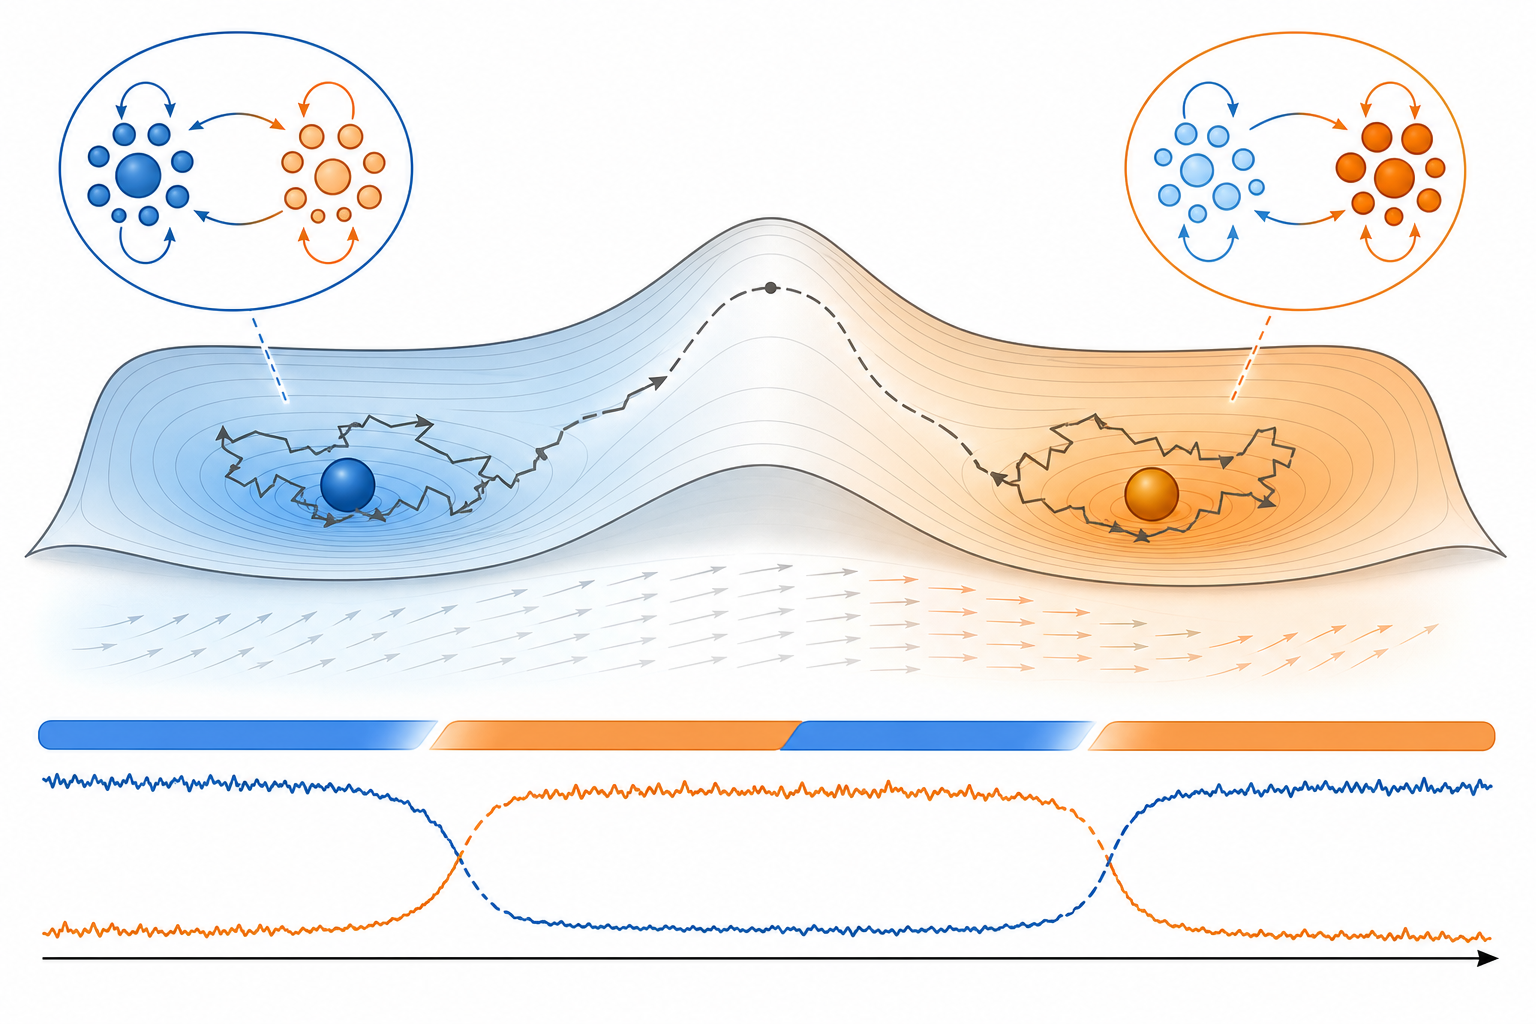
\includegraphics[width=0.92\textwidth]{figures/mhbf-bistable-attractor-switching.png}
\caption{Bistable perception can be pictured as motion between two attractor basins. Competition makes one percept dominate at a time; slow adaptation reshapes the currently occupied basin; noise can then push the state across the barrier into the other interpretation.}
\end{figure}

\subsection{A two-population competition model}

A minimal rate model uses two activity variables, \(u_1(t)\) and \(u_2(t)\), for the two perceptual populations:
\[
\tau_u \frac{d u_1}{dt}
=
-u_1
+ f(\alpha u_1-\beta u_2-a_1+I_1),
\]
\[
\tau_u \frac{d u_2}{dt}
=
-u_2
+ f(\alpha u_2-\beta u_1-a_2+I_2).
\]
Here \(I_i\) is sensory drive to population \(i\), \(\alpha>0\) is recurrent self-excitation, \(\beta>0\) is mutual inhibition, \(a_i\) is adaptation, and \(f\) is a threshold nonlinearity such as a Heaviside or sigmoid function.

Each term has a distinct role:
\begin{itemize}
    \item \(I_i\) says how strongly the stimulus supports interpretation \(i\).
    \item \(\alpha u_i\) stabilizes the active interpretation by recurrent excitation.
    \item \(-\beta u_j\) suppresses the competing interpretation.
    \item \(-a_i\) slowly weakens the currently dominant population.
\end{itemize}

With a hard threshold \(f\), the perceptual fixed points of interest are approximately
\[
(u_1,u_2)\approx(1,0)
\qquad\text{or}\qquad
(u_1,u_2)\approx(0,1).
\]
These correspond to percept \(A\) on or percept \(B\) on. Mutual inhibition makes the mixed state harder to maintain, while self-excitation makes the current dominant state persistent.

\begin{figure}[!htbp]
\centering
\begin{tikzpicture}[>=Latex, thick]
    \tikzstyle{pop}=[draw, circle, minimum size=1.35cm, align=center]
    \tikzstyle{box}=[draw, rounded corners, align=center, minimum height=0.8cm, inner sep=5pt]

    \node[box] (s1) at (-3.7,-1.9) {stimulus\\drive \(I_1\)};
    \node[box] (s2) at (3.7,-1.9) {stimulus\\drive \(I_2\)};
    \node[pop] (u1) at (-1.7,0) {\(u_1\)\\\(a_1\)};
    \node[pop] (u2) at (1.7,0) {\(u_2\)\\\(a_2\)};
    \node[box] (p1) at (-1.7,1.9) {percept \(A\)};
    \node[box] (p2) at (1.7,1.9) {percept \(B\)};

    \draw[->] (s1) -- (u1);
    \draw[->] (s2) -- (u2);
    \draw[->] (u1) -- (p1);
    \draw[->] (u2) -- (p2);

    \draw[->] (u1.135) .. controls (-2.8,1.1) and (-0.6,1.1) .. (u1.45);
    \draw[->] (u2.135) .. controls (0.6,1.1) and (2.8,1.1) .. (u2.45);
    \node at (-1.7,1.05) {\(\alpha\)};
    \node at (1.7,1.05) {\(\alpha\)};

    \draw[->] (u1.15) .. controls (0.0,0.78) and (0.0,0.78) .. (u2.165);
    \draw[->] (u2.195) .. controls (0.0,-0.78) and (0.0,-0.78) .. (u1.345);
    \node at (0,1.05) {\(\beta\)};
    \node at (0,-1.05) {\(\beta\)};

    \node[align=center] at (0,-2.95) {self-excitation stabilizes each percept; mutual inhibition prevents both from dominating together};
\end{tikzpicture}
\caption{Two-population competition model for bistable perception. The variables \(u_1,u_2\) are fast activities, while \(a_1,a_2\) are slower adaptation variables that weaken the currently active population.}
\end{figure}

\subsection{Mechanism 1: adaptation as a deterministic switch}

Adaptation means that a strongly active population becomes less effective over time. This can be implemented as neuronal fatigue or synaptic depression. A simple adaptation equation is
\[
\tau_a \frac{d a_i}{dt}
=
-a_i + \gamma u_i,
\qquad
\tau_a \gg \tau_u .
\]
The time-scale separation is the key. Activity \(u_i\) changes quickly, but adaptation \(a_i\) accumulates slowly. If percept \(A\) is dominant, then \(u_1\) is high and \(a_1\) gradually increases. The effective input to population \(A\),
\[
\alpha u_1-\beta u_2-a_1+I_1,
\]
therefore decreases. Once this input falls below the threshold needed to maintain \(A\), population \(B\) can escape suppression and become dominant.

This produces an oscillator-like model of perceptual alternation:
\[
A \text{ dominates}
\rightarrow A \text{ adapts}
\rightarrow B \text{ takes over}
\rightarrow B \text{ adapts}
\rightarrow A \text{ returns}.
\]
The strength of the adaptation model is that it explains why switches happen even without external stimulus changes. Its weakness is that a purely deterministic oscillator tends to produce too-regular alternations. Real percept durations are variable.

\subsection{Percept durations and the gamma distribution}

The lecture emphasizes that percept durations are often fit by a gamma distribution:
\[
p(T)
=
\frac{1}{\tau^k \Gamma(k)}
T^{k-1}e^{-T/\tau},
\qquad
T>0.
\]
The parameter \(k\) controls the shape, and \(\tau\) sets the time scale. The mean and variance are
\[
\mathbb{E}[T]=k\tau,
\qquad
\operatorname{Var}(T)=k\tau^2.
\]

This is a useful diagnostic. A deterministic oscillator would predict a narrow distribution centered near one period. White-noise escape from a fixed attractor would often predict an exponential distribution,
\[
p(T)=\lambda e^{-\lambda T},
\]
which is the special memoryless case. The gamma-like empirical shape suggests that switching is neither perfectly clocklike nor simply memoryless. It often looks like adaptation changes the barrier slowly, while noise supplies the final push.

\begin{figure}[!htbp]
\centering
\begin{tikzpicture}[>=Latex, thick]
    \begin{axis}[
        width=0.78\textwidth,
        height=5.2cm,
        xlabel={percept duration \(T\)},
        ylabel={density},
        xmin=0, xmax=7,
        ymin=0, ymax=0.75,
        axis lines=left,
        legend style={draw=none, at={(0.98,0.95)}, anchor=north east},
        every axis plot/.append style={line width=1.1pt},
        samples=180
    ]
        \addplot[black, dashed, domain=0:7] {0.65*exp(-0.65*x)};
        \addlegendentry{noise-only exponential}
        \addplot[black, domain=0:7] {(x^2)*exp(-x)/2};
        \addlegendentry{gamma-like switching}
    \end{axis}
\end{tikzpicture}
\caption{Percept-duration distributions help distinguish mechanisms. A fixed-barrier noise model gives memoryless exponential escape times. Adaptation plus noise naturally produces a more peaked, gamma-like distribution because the escape probability changes with time since the last switch.}
\end{figure}

\subsection{Mechanism 2: noise-driven attractor transitions}

The second mechanism is noise. Neural activity fluctuates. Even if percept \(A\) is currently dominant, a fluctuation can make \(A\) temporarily less suppressive or make \(B\) temporarily stronger. If the fluctuation is large enough, the system crosses the boundary between attractors.

A compact one-dimensional description uses a state variable
\[
r = r_A-r_B,
\]
where \(r>0\) means percept \(A\) dominates and \(r<0\) means percept \(B\) dominates. A stochastic attractor model can be written as
\[
dr_t
=
-\frac{\partial E(r_t)}{\partial r}\,dt
+\sigma\,dW_t .
\]
The energy function \(E(r)\) has two minima. The noise term \(dW_t\) is Brownian motion, and \(\sigma\) controls fluctuation strength.

\begin{figure}[!htbp]
\centering
\begin{tikzpicture}[>=Latex, thick]
    \begin{axis}[
        width=0.72\textwidth,
        height=5.1cm,
        xlabel={state \(r=r_A-r_B\)},
        ylabel={energy \(E(r)\)},
        xmin=-2.2, xmax=2.2,
        ymin=-0.4, ymax=4.2,
        axis lines=left,
        xtick={-1,0,1},
        xticklabels={\(B\) on, barrier, \(A\) on},
        ytick=\empty,
        samples=180
    ]
        \addplot[black, domain=-2.1:2.1] {(x^2-1)^2};
        \addplot[black, mark=*] coordinates {(-1,0) (1,0)};
        \addplot[black, dashed, ->] coordinates {(-1,0.15) (-0.55,0.45) (-0.2,0.95) (0.15,1.12) (0.55,0.45) (1,0.15)};
    \end{axis}
\end{tikzpicture}
\caption{Attractor picture for noise-driven switching. The system usually sits near one energy minimum. A large enough fluctuation can move it over the barrier into the other basin. Adaptation lowers the effective barrier for the currently dominant percept.}
\end{figure}

This model makes two intuitions explicit:
\begin{itemize}
    \item stable percepts are local minima of a neural energy or potential landscape;
    \item perceptual switches are barrier-crossing events.
\end{itemize}

Moreno-Bote, Rinzel, and Rubin's account combines the two mechanisms: adaptation alone is not strong enough to force every transition, but it reduces the barrier so that noise-triggered transitions become more likely. That hybrid model explains both persistence and variability.

\subsection{Bayesian sampling interpretation}

The Bayesian sampling view reframes bistability as approximate inference. Let \(h\) denote a possible perceptual interpretation and \(s\) the sensory data. The posterior distribution is
\[
p(h\mid s)
\propto
p(s\mid h)p(h).
\]
For an ambiguous stimulus, the posterior may be multimodal: two or more interpretations have high probability. Perceptual experience may then resemble a sequence of samples from this posterior rather than a single maximizer.

In that view, alternations are not a failure of perception. They are a possible signature of uncertainty. If two interpretations explain the sensory data nearly equally well, a sampling system should sometimes visit both.

\paragraph{Connection.}
Attractor models and sampling models are not opposites. A neural attractor can implement a mode of the posterior, while noise-driven transitions between attractors can approximate sampling across modes. The same mechanism can therefore be read dynamically or probabilistically.

\subsection{Multisensory integration as inference}

The second half of the lecture turns to a different ambiguity: different sensory modalities provide different noisy measurements of the same world property. For example, vision and touch can both provide information about object size. The problem is to infer the hidden world state \(h\) from sensory observations \(s_1\) and \(s_2\).

The generative model is
\[
h \sim p(h),
\qquad
s_1 \sim p(s_1\mid h),
\qquad
s_2 \sim p(s_2\mid h).
\]
Bayes' rule gives
\[
p(h\mid s_1,s_2)
=
\frac{p(s_1,s_2\mid h)p(h)}
{p(s_1,s_2)}.
\]
If the two sensory noise sources are conditionally independent given the world state, then
\[
p(s_1,s_2\mid h)
=
p(s_1\mid h)p(s_2\mid h).
\]

\begin{figure}[!htbp]
\centering
\begin{tikzpicture}[>=Latex, thick, node distance=1.0cm and 1.3cm]
    \tikzstyle{box}=[draw, rounded corners, align=center, minimum height=0.82cm, inner sep=5pt]
    \node[box] (prior) {prior \(p(h)\)};
    \node[box, below=of prior] (world) {hidden world\\state \(h\)};
    \node[box, below left=of world] (s1) {cue 1\\\(s_1\)};
    \node[box, below right=of world] (s2) {cue 2\\\(s_2\)};
    \node[box, below=1.2cm of world, minimum width=5.4cm] (post) {posterior \(p(h\mid s_1,s_2)\)};
    \node[box, below=of post] (estimate) {estimate \(\hat h\)};

    \draw[->] (prior) -- (world);
    \draw[->] (world) -- node[left] {\(p(s_1\mid h)\)} (s1);
    \draw[->] (world) -- node[right] {\(p(s_2\mid h)\)} (s2);
    \draw[->] (s1) -- (post);
    \draw[->] (s2) -- (post);
    \draw[->] (post) -- (estimate);
\end{tikzpicture}
\caption{Generative model for cue integration. The world state causes sensory measurements, and inference runs in the opposite direction: combine the cues to estimate the hidden state.}
\end{figure}

\subsection{Maximum-likelihood cue combination}

The lecture derives the maximum-likelihood estimate under three assumptions:
\begin{itemize}
    \item the prior is flat, so all values of \(h\) are initially equally plausible;
    \item each cue is Gaussian around the true state;
    \item the noise in the two cues is independent.
\end{itemize}

Write the likelihoods as
\[
p(s_i\mid h)
=
\frac{1}{\sqrt{2\pi\sigma_i^2}}
\exp\!\left[-\frac{(s_i-h)^2}{2\sigma_i^2}\right],
\qquad i\in\{1,2\}.
\]
The negative log-likelihood, ignoring constants, is
\[
\mathcal L(h)
=
\frac{(s_1-h)^2}{2\sigma_1^2}
+
\frac{(s_2-h)^2}{2\sigma_2^2}.
\]
Minimizing \(\mathcal L\) gives
\[
\frac{\partial \mathcal L}{\partial h}
=
\frac{h-s_1}{\sigma_1^2}
+
\frac{h-s_2}{\sigma_2^2}
=0.
\]
Let the precision of cue \(i\) be
\[
p_i=\frac{1}{\sigma_i^2}.
\]
Then the estimate is
\[
\hat h
=
\frac{p_1}{p_1+p_2}s_1
+
\frac{p_2}{p_1+p_2}s_2.
\]

The rule is simple: each cue is weighted by its reliability. A cue with low variance has high precision and receives a larger weight. A cue with high variance has low precision and receives a smaller weight.

\[
\boxed{
\hat h
=
w_1s_1+w_2s_2,
\qquad
w_i=\frac{p_i}{p_1+p_2},
\qquad
p_i=\frac{1}{\sigma_i^2}
}
\]
Here \(\hat h\) is the maximum-likelihood estimate of the hidden state, \(s_i\) are the sensory measurements, \(w_i\) are reliability weights, and \(p_i\) are precisions.

\subsection{Why combined estimates are more precise}

The combined posterior is also narrower than either individual likelihood. For independent Gaussian cues, precisions add:
\[
p_{1+2}=p_1+p_2.
\]
Equivalently,
\[
\sigma_{1+2}^2
=
\frac{1}{p_1+p_2}
=
\frac{1}{1/\sigma_1^2+1/\sigma_2^2}.
\]
Because \(p_1+p_2\) is larger than either precision alone, the combined variance is smaller than either single-cue variance.

\begin{figure}[!htbp]
\centering
\begin{tikzpicture}[>=Latex, thick]
    \begin{axis}[
        width=0.78\textwidth,
        height=5.2cm,
        xlabel={state \(h\)},
        ylabel={relative likelihood},
        xmin=-3.2, xmax=3.2,
        ymin=0, ymax=1.25,
        axis lines=left,
        legend style={draw=none, at={(0.03,0.95)}, anchor=north west},
        every axis plot/.append style={line width=1.1pt},
        samples=180
    ]
        \addplot[black, dashed, domain=-3.2:3.2] {exp(-((x+0.75)^2)/(2*1.15^2))};
        \addlegendentry{noisier cue}
        \addplot[black, dotted, domain=-3.2:3.2] {exp(-((x-0.55)^2)/(2*0.55^2))};
        \addlegendentry{reliable cue}
        \addplot[black, domain=-3.2:3.2] {1.12*exp(-((x-0.32)^2)/(2*0.50^2))};
        \addlegendentry{combined estimate}
    \end{axis}
\end{tikzpicture}
\caption{Gaussian cue combination. The combined estimate lies closer to the more reliable cue and has lower variance than either cue alone.}
\end{figure}

This is the core normative prediction of multisensory integration: if the nervous system combines cues optimally, then behavior should show both reliability-weighted bias and improved discrimination precision.

\subsection{Psychometric functions, PSEs, and thresholds}

The slides connect the model to psychophysical reports. In a typical task, an observer judges whether a comparison stimulus is wider or taller than a reference. Across many trials, the proportion of ``comparison is larger'' responses defines a psychometric curve.

A standard model is
\[
P(\text{respond ``comparison larger''}\mid x)
=
\Phi\left(\frac{x-\mu}{\sigma_{\mathrm{psy}}}\right),
\]
where \(x\) is the comparison value, \(\Phi\) is the Gaussian cumulative distribution function, \(\mu\) is the point of subjective equality (PSE), and \(\sigma_{\mathrm{psy}}\) controls the slope.

These parameters have direct meanings:
\begin{itemize}
    \item the \textbf{PSE} tells us which comparison value feels equal to the standard, so PSE shifts reveal cue weighting and perceptual bias;
    \item the \textbf{threshold} is related to the inverse slope, so a smaller threshold means finer discrimination.
\end{itemize}

The theory therefore predicts two measurable effects when cue reliability changes:
\begin{itemize}
    \item the more reliable cue should receive more weight, shifting the PSE appropriately;
    \item the bimodal threshold should improve relative to either unimodal threshold.
\end{itemize}

\subsection{The Ernst and Banks result}

The lecture discusses the classic visual--haptic experiments of Ernst and Banks. Subjects judged object properties in conditions where visual reliability could be manipulated while haptic reliability remained available. The experiment followed a clean logic:
\begin{enumerate}
    \item measure unimodal visual thresholds at several visual noise levels;
    \item measure unimodal haptic thresholds;
    \item convert those thresholds into variance or precision estimates;
    \item predict the bimodal weights and thresholds from the maximum-likelihood rule;
    \item compare the predictions with observed bimodal behavior.
\end{enumerate}

The central result is that humans often combine visual and haptic information in a statistically near-optimal way. As visual noise increases, the visual weight decreases and the haptic weight increases. The combined threshold is typically close to the value predicted by the sum of unimodal precisions.

This makes the theory experimentally meaningful: the precision-weighted fusion rule is not just mathematically convenient, it is behaviorally testable.

\subsection{Common misunderstanding: averaging is not enough}

It is tempting to summarize multisensory integration as ``the brain averages the senses.'' That is incomplete. The model says the system computes a \emph{weighted} average, and the weights are not arbitrary:
\[
w_{\mathrm{visual}}
=
\frac{1/\sigma_{\mathrm{visual}}^2}
{1/\sigma_{\mathrm{visual}}^2+1/\sigma_{\mathrm{haptic}}^2},
\qquad
w_{\mathrm{haptic}}
=
\frac{1/\sigma_{\mathrm{haptic}}^2}
{1/\sigma_{\mathrm{visual}}^2+1/\sigma_{\mathrm{haptic}}^2}.
\]
The weights should change dynamically when the reliability of a modality changes. That is why adding visual noise should reduce visual weight and increase haptic weight.

\subsection{When the cues disagree too much}

The precision-weighted average assumes that the cues arise from the same hidden cause and should therefore be fused. But this assumption can fail. If the visual and haptic cues disagree too strongly, the more important question is not how to weight them but whether they should be integrated at all.

A robust formulation introduces a latent causal variable \(C\) indicating whether the cues share a common source:
\[
P(h,C\mid s_1,s_2) \propto P(s_1,s_2\mid h,C)P(h\mid C)P(C).
\]
Under \(C=1\), the cues are fused. Under \(C=0\), they are treated as arising from distinct causes and may be kept separate or one may be discounted.

The conceptual lesson is important: optimal fusion is the right rule only \emph{after} deciding that the cues belong together. Causal inference decides whether fusion should happen in the first place.

\subsection{How the two halves of the lecture fit together}

Bistability and multisensory integration both concern inference under uncertainty, but they emphasize different posterior shapes.

\begin{center}
\begin{tabular}{lp{0.58\textwidth}}
\hline
Case & Modeling picture \\
\hline
Bistable perception & posterior or energy landscape has multiple strong interpretations; dynamics and noise determine which mode is experienced now \\
Multisensory integration & cues support a common hidden state; independent Gaussian evidence combines by adding precision \\
Adaptation & slowly changes the landscape so the current percept becomes less stable \\
Noise & causes stochastic transitions or trial-to-trial variability in estimates \\
Reliability weighting & gives more influence to cues with lower variance \\
\hline
\end{tabular}
\end{center}

The shared lesson is that perception is active model selection. Sometimes the model must choose between incompatible interpretations. Sometimes it must fuse compatible measurements. In both cases, a higher-brain model is useful when it specifies the hidden state, the sensory evidence, the uncertainty, and the dynamics or decision rule that connects them.

\subsection{Conceptual takeaways from Lecture 3}

\begin{itemize}
    \item Ambiguous stimuli can produce alternating percepts because competing neural populations inhibit one another.
    \item Adaptation weakens the currently dominant perceptual population and can create oscillatory switching.
    \item Noise explains variability in percept durations and can push the system between attractor basins.
    \item Adaptation plus noise is more realistic than either mechanism alone for many bistable-perception data.
    \item Bayesian sampling treats perceptual alternations as sequential samples from a multimodal posterior.
    \item Multisensory integration can be modeled as inference about a hidden world state from multiple sensory cues.
    \item Under independent Gaussian noise and a flat prior, the maximum-likelihood estimate is a precision-weighted average.
    \item Optimal cue integration predicts both reliability-dependent cue weights and lower bimodal variance.
    \item Large cue discrepancies require causal inference, because the first question becomes whether the cues should be fused at all.
\end{itemize}

\subsection*{Sources mentioned in Lecture 3}

\begin{itemize}
    \item C. R. Laing and C. C. Chow (2002), oscillator models of binocular rivalry and perceptual alternations.
    \item J. W. Brascamp and colleagues (2005), work on percept-duration distributions in bistable perception.
    \item R. Moreno-Bote, J. Rinzel, and N. Rubin (2007), combined adaptation-and-noise account of perceptual switching.
    \item S. J. Gershman, E. Vul, and J. B. Tenenbaum (2012), Bayesian and sampling interpretations of perception.
    \item P. R. Schrater and R. Sundareswara (2006), sampling models of perceptual inference.
    \item M. O. Ernst and M. S. Banks (2002), ``Humans integrate visual and haptic information in a statistically optimal fashion,'' \emph{Nature}.
\end{itemize}
